% ============================ SITE ==================================
\phase{Phase two \textbullet\ Where}{Choosing the site with a method, not a hunch}{Four coastal hubs, six criteria, and a test of how easily the answer flips.}\label{sec:site}

Location is the one operations decision you cannot undo. We used the \textbf{Analytic Hierarchy Process (AHP)}, a standard tool for choosing between sites \cite{saaty1980}. It works in three steps. First, we compare the criteria two at a time (``is being near the buyer more important than being near the port, and by how much?'') on a 1--9 scale. Second, a little matrix algebra turns those comparisons into weights and checks that our judgements do not contradict each other. Third, we score each site on each criterion and add up the weighted scores.

\subsection{The weights}
\begin{center}\tablefont
\begin{tabularx}{\textwidth}{@{}l c L@{}}
\toprule
\thead{Criterion} & \thead{Weight} & \thead{Why it matters for \emph{our} product}\\ \midrule
Anchor buyers nearby & 33.3\% & Hydrogen is costly to move. A buyer within a short pipeline run removes trucks, compression and a whole layer of risk.\\
Renewable resource & 19.5\% & Power is about half of our cost. Better sun and wind means fewer megawatts to buy and a higher electrolyser load.\\
Grid and transmission & 19.5\% & We bring solar and wind power across the state over the national grid; a weak node delays connection.\\
Port and export & 10.7\% & Matters for phase two (ammonia) and for importing stacks.\\
Land and state policy & 10.7\% & Land cost, speed of clearances, state incentives.\\
Water & 6.4\% & About 9 litres of pure water per kg in the reaction alone, more once purification and cooling are counted \cite{rmi2023}; small in cost but sensitive locally.\\
\bottomrule
\end{tabularx}
\end{center}
The consistency ratio is \textbf{0.006}, far below the 0.10 ceiling Saaty set \cite{saaty1980}. In plain words, our pairwise judgements hang together; we did not, for example, say A beats B, B beats C and C beats A. \confH\ (for the arithmetic; the judgements themselves are ours, so \confM.)

\subsection{The scores and the result}
\begin{center}\tablefont
\begin{tabularx}{\textwidth}{@{}l c c c c c c L@{}}
\toprule
\thead{Site} & \thead{Buyers} & \thead{RE} & \thead{Port} & \thead{Water} & \thead{Land} & \thead{Grid} & \thead{The reason in one line}\\ \midrule
\textbf{Paradip} & 9 & 5 & 8 & 7 & 7 & 7 & IOCL refinery, IFFCO and Paradeep Phosphates within a few km; Odisha wind is weak.\\
Kandla & 6 & 9 & 8 & 4 & 8 & 8 & Best solar and wind in India; but IFFCO Kandla buys ammonia, and the refineries sit across the Gulf of Kutch; water-stressed.\\
Kakinada & 6 & 7 & 7 & 7 & 7 & 7 & Coromandel nearby; a crowded green-ammonia cluster competing for land and power.\\
Tuticorin & 5 & 8 & 8 & 6 & 7 & 6 & Strong Tamil Nadu wind; few anchor buyers for hydrogen itself.\\
\bottomrule
\end{tabularx}
\end{center}

\begin{figure}[H]
\centering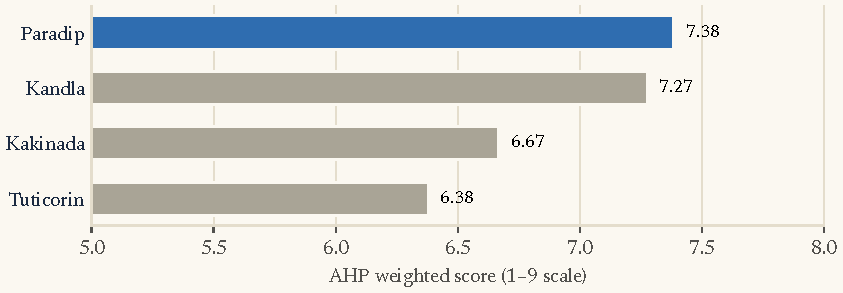
\includegraphics[width=\textwidth]{site_ahp.pdf}
\caption{AHP weighted scores. Paradip wins, but only just. Source: our model, \texttt{siteselect.py}.}
\end{figure}

\subsection{How fragile is the answer?}
A ranking is only as good as its closest call. We asked: \emph{how low would the weight on ``buyers nearby'' have to fall before Kandla wins?} The answer is \textbf{30.8\%}, against the 33.3\% we chose. A shift of 2.5 percentage points flips the decision.

\begin{finding}[What the site analysis really says]
The site depends on the product. \textbf{If we sell hydrogen, Paradip wins, because the buyer is next door. If we sell ammonia or export, Kandla wins, because cheap power then matters more than proximity.} That is why we wrote the product decision first. It also tells us what to watch: if the Paradip refinery will not sign, we should not ``make Paradip work''; we should move the project to the best-power site and change the product. \confM
\end{finding}

\begin{plainwords}[A local wrinkle]
Paradip is not empty. The lowest green-ammonia bid in India's 2025 auctions, ₹49.75/kg, was for IFFCO at Paradeep \cite{seci2025}. A cluster brings shared pipelines and skilled workers, but also competition for the same land, water and transmission capacity. We treat ``cluster congestion'' as a named risk in Section~\ref{sec:risk}.
\end{plainwords}
\newpage
